\section*{APPENDIX}
\subsection*{A. Text Explainer}\label{appendix:textexplainer}
\begin{figure}[h]
	\centering
	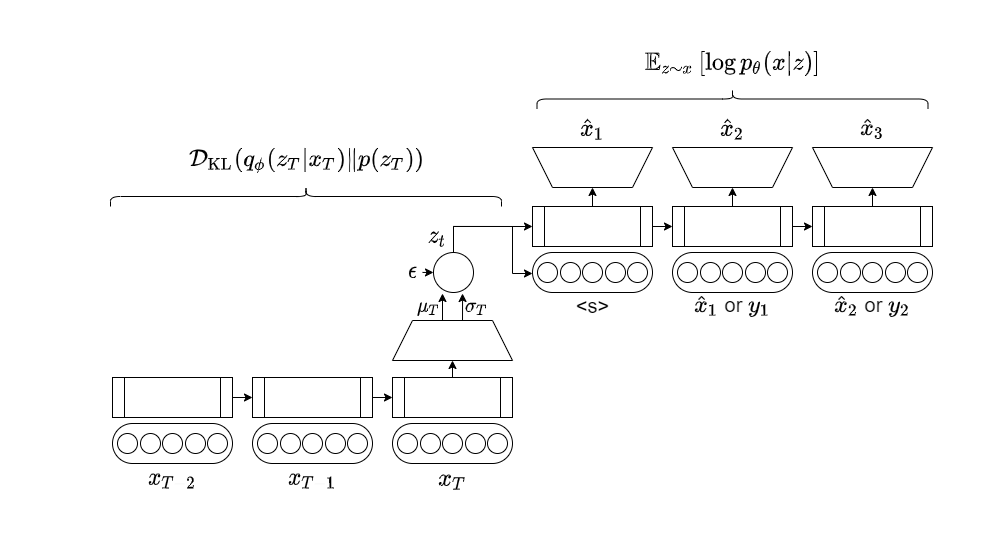
\includegraphics[width=\textwidth]{../openreview/pictures/TextVaewithHolisticRegularization.png}
	\caption{Text-VAE architecture.}
	\label{fig:TextVAE}
\end{figure}

%\begin{table}[t]
%    \centering
%    \caption{Samples drawn from the Text-VAE and the GCE that was trained from it.}
%    \begin{minipage}{1\linewidth}
%    \begin{tabular}{p{0.45\textwidth}|p{0.45\textwidth}}
%        \toprule \\
%        Text-VAE & Text-GCE \\
%        \midrule
%        plays like an unbalanced mixture of flavours and violence   the movie unfolds with an undeniable mixture of %dignity that sneaks up in the viewer & -2.00: but and heartwarming   it does and involving    and involving    and involving    and evocative visuals and \\
%        & -1.00: but and heartwarming   it does          and involving    and involving    and involving and involving \\
%        highlighted by a gritty cast   but it makes you feel like a character   but ends up as shallow and unsettling as one & 0.00: but and it works and ponderous and romantic flicks and clich and \\
%        & +1.00: but and it works and ponderous and snipes and romantic flicks and clich\\
%        at times a bit melodramatic   it would be a bit better than you  d expect if you  ve never seen it all before & +2.00: but and heartwarming  it does and clich and clich and clich \\
%        \bottomrule
%    \end{tabular}
%    \label{tab:TextVAE}
%    \end{minipage}
%\end{table}

The text classifier used a bi-directional LSTM of 256 units. As mentioned the embeddings had been initialised using pre-trained GLoVe embeddings. All hidden states were then concatenated into a single feature map. Blocks of convolutional layers (32 filters of kernel size 3), ReLU activations and max-pooling (kernel size of 2 and stide of 2) were applied to reduce these feature map sizes. Ultimately all feature maps were projected down into the required number of classes using a linear layer. Adam was used as the optimizer, using an initial learning rate of 1e-3 and decaying this by a factor of 0.85 at every epoch.

The text-VAE follows the proposed structure given in \cite{he2019lagging} as closely as possible. The embeddings used 512 dimensions and the single layer LSTM 1024. The last hidden and cell states were projected down to 32 latent dimensions. Aggressive training was used until the mutual information between the latent variables and the encoder input stabilised (typically 5 epochs). For the inner loop in the aggressive training schedule, 250 iterations were allowed, after which it was assumed the encoder had converged. The Kullback-Leibler divergence was weighted using a linear annealing schedule between the first 10 epochs. 

Fine-tuning was attempted using $\lambda=1-3$ and $lr=1e-3$ using the standard GCE training scheme. These hyperparameters empirically proved to induce lowest lowest causal loss after a gridsearch. Ultimately, no model improved it's causal loss after more than 3 epochs.

\subsection*{B. Neural network architectures}\label{appendix:architectures}
\begin{table}[h]
	\centering
	\caption{Network architecture for CNN classifier}\label{tab:cnn_architecture}
	\begin{tabular}{|c|}
		\toprule[1.5pt]
		Network architecture for CNN classifier\\
		\hline
		Input (28×28)\\
		Conv2 (32 channels, 3×3 kernels, stride 1, pad 0) \\
		ReLU\\
		Conv2 (64 channels, 3×3 kernels, stride 1, pad 0) ReLU\\
		MaxPool (2×2 kernel)\\
		Dropout (p = 0.5)\\
		Linear (128 units)\\
		ReLU\\
		Dropout (p = 0.5)\\
		Linear (M units)
		Softmax\\
		\hline
	\end{tabular}
	
	\caption{GCE network architecture used for MNIST and fMNIST experiments}\label{tab:gce_architecture}
	\begin{tabular}{|c|c|}
		\toprule[1.5pt]
		Encoder & Decoder\\
		\hline
		Input (28×28) & Input (K + L)\\
		Conv2 (64 chan., 4×4 kernels, stride 2, pad 1) & Linear (3136 units)\\
		ReLU& ReLU\\
		Conv2 (64 chan., 4×4 kernels, stride 2, pad 1) & Conv2T (64 chan., 4×4, 1, 1)\\
		ReLU& ReLU\\
		Conv2 (64 chan., 4×4 kernels, stride 1, pad 0) & Conv2T (64 chan., 4×4, 2, 2)\\
		ReLU& ReLU\\
		Linear (K + L units for both $\mu$ and $\sigma$)& Conv2T (1 chan., 4×4, 2, 1)\\
		& Sigmoid\\
		\hline
	\end{tabular}
	\begin{minipage}{0.45\linewidth}
		\centering
		\caption{Hyperparameter settings for GCE models}\label{tab:hyperparameter_gce}
		\begin{tabular}{l |c c c}
			\toprule
			\multicolumn{1}{c}{} & \multicolumn{3}{|c}{Dataset}\\
			\cline{2-4}
			\multicolumn{1}{c}{}&\multicolumn{1}{|c}{MNIST}  & \multicolumn{1}{c}{MNIST}  & \multicolumn{1}{c}{FMNIST} \\
			\midrule
			{\tiny classes} & 3,8 & 1,4,9 & 0,3,4\\ 
			K & 1 &  2  &2  \\
			L & 7& 2 & 4\\
			$\lambda$  & 0.05 & 0.1 & 0.05\\
			steps & 8000 & 8000 & 8000\\
			lr & $5 \times 10^{-4}$ & $5 \times 10^{-4}$ & $10^{-4}$\\
			$N\alpha$ & 100 & 75 & 100\\
			$N\beta$ &  25 & 25 & 25\\
			{\tiny batch size} &  64 & 64 & 32\\
			\bottomrule
		\end{tabular}
	\end{minipage}
	\hspace{1cm}
	\begin{minipage}{0.45\linewidth}
		\centering
		\caption{Hyperparameter settings for CNN classifier}\label{tab:hyperparameter_cnn}
		\begin{tabular}{l |c c c}
			\toprule
			\multicolumn{1}{c}{} & \multicolumn{3}{|c}{Dataset}\\
			\cline{2-4}
			\multicolumn{1}{c}{ }&\multicolumn{1}{|c}{MNIST}  & \multicolumn{1}{c}{MNIST}  & \multicolumn{1}{c}{FMNIST} \\
			\midrule
			{\tiny classes} & 3,8 & 1,4,9 & 0,3,4\\ 
			lr &  0.1 & 0.1 & 0.1\\
			mom. &   0.5& 0.5& 0.5\\
			{\tiny batch size} &  64& 64&64\\
			epochs &  20 & 30 & 50 \\
			\bottomrule
		\end{tabular}
	\end{minipage}
\end{table}

\newpage
\subsection*{C. Additional Reproduction results}\label{appendix:additionalresults}
\begin{figure}[h]
	\centering
	\begin{subfigure}[t]{.23\linewidth}
		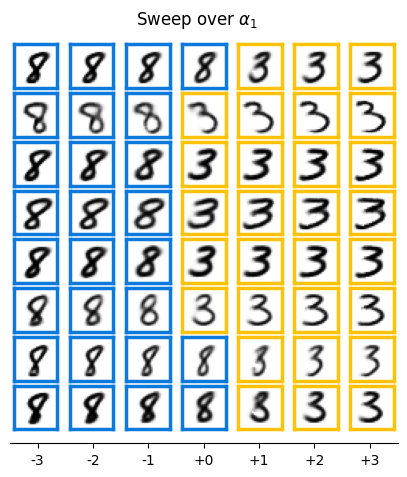
\includegraphics[width=.9\textwidth]{../openreview/pictures/Figure3/alpha_1.png}
		\caption{Sweep $\alpha_1$}
		% \label{fig:alpha_1}
	\end{subfigure}
	\begin{subfigure}[t]{.23\linewidth}
		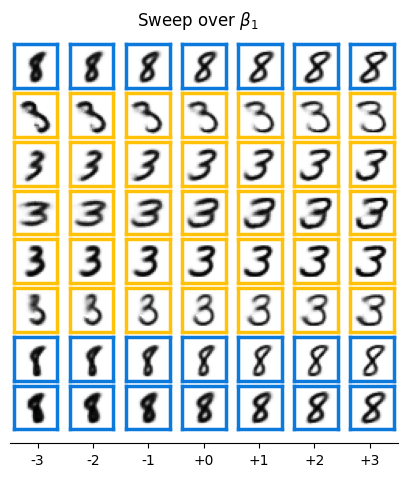
\includegraphics[width=.9\textwidth]{../openreview/pictures/Figure3/beta_1.png}
		\caption{Sweep $\beta_1$}
		% \label{fig:beta_1}
	\end{subfigure}
	\begin{subfigure}[t]{.23\linewidth}
		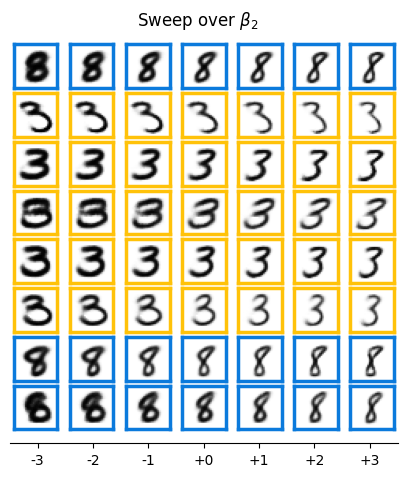
\includegraphics[width=.9\textwidth]{../openreview/pictures/Figure3/beta_2.png}
		\caption{Sweep $\beta_2$}
		% \label{fig:beta_1}
	\end{subfigure}
	\begin{subfigure}[t]{.23\linewidth}
		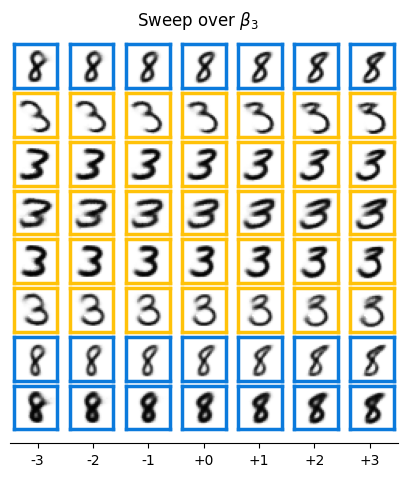
\includegraphics[width=.9\textwidth]{../openreview/pictures/Figure3/beta_3.png}
		\caption{Sweep $\beta_3$}
		% \label{fig:beta_2}
	\end{subfigure}
	\begin{subfigure}[t]{.23\linewidth}
		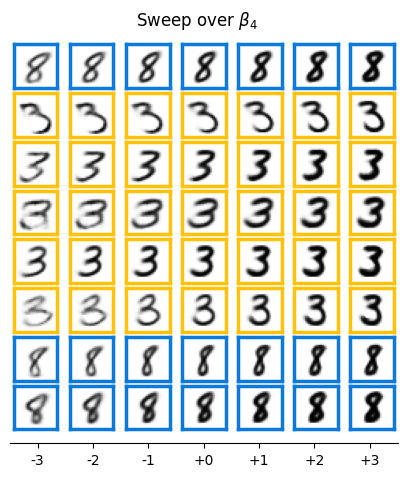
\includegraphics[width=.9\textwidth]{../openreview/pictures/Figure3/beta_4.png}
		\caption{Sweep $\beta_4$}
		% \label{fig:beta_2}
	\end{subfigure}
	\begin{subfigure}[t]{.23\linewidth}
		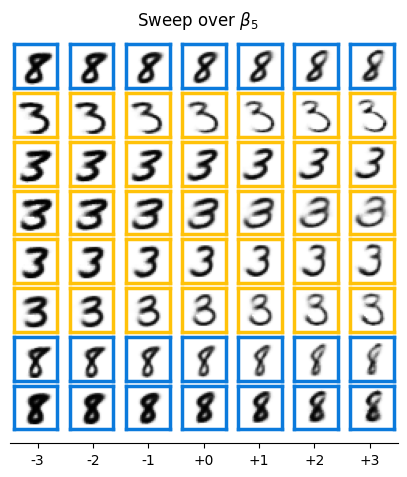
\includegraphics[width=.9\textwidth]{../openreview/pictures/Figure3/beta_5.png}
		\caption{Sweep $\beta_5$}
		% \label{fig:beta_2}
	\end{subfigure}
	\begin{subfigure}[t]{.23\linewidth}
		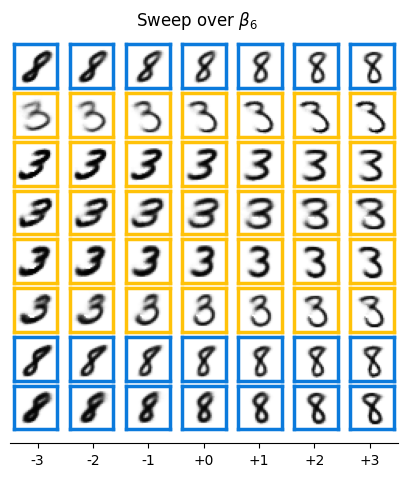
\includegraphics[width=.9\textwidth]{../openreview/pictures/Figure3/beta_6.png}
		\caption{Sweep $\beta_6$}
		% \label{fig:beta_2}
	\end{subfigure}
	\begin{subfigure}[t]{.23\linewidth}
		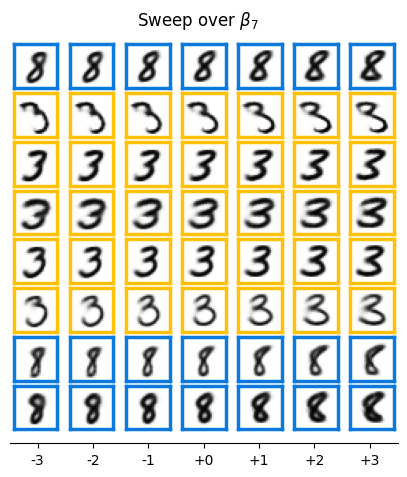
\includegraphics[width=.9\textwidth]{../openreview/pictures/Figure3/beta_7.png}
		\caption{Sweep $\beta_7$}
		% \label{fig:beta_2}
	\end{subfigure}
	\caption{Visualizations of learned latent factors for MNIST classifier trained on classes '3' \& '8'}
	\label{fig:complte_:mnist_results 38}
	
	\begin{subfigure}[t]{.23\linewidth}
		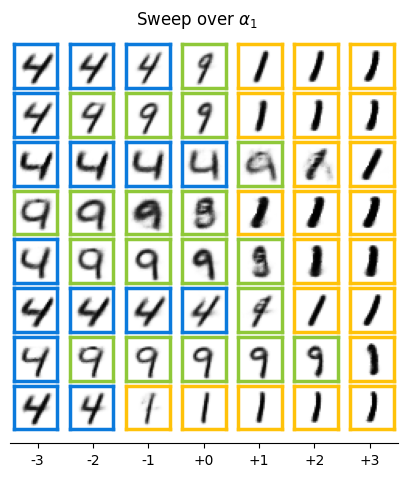
\includegraphics[width=.9\textwidth]{../openreview/pictures/Figure13/alpha_1.png}
		\caption{Sweep $\alpha_1$}
		% \label{fig:alpha_1}
	\end{subfigure}
	\begin{subfigure}[t]{.23\linewidth}
		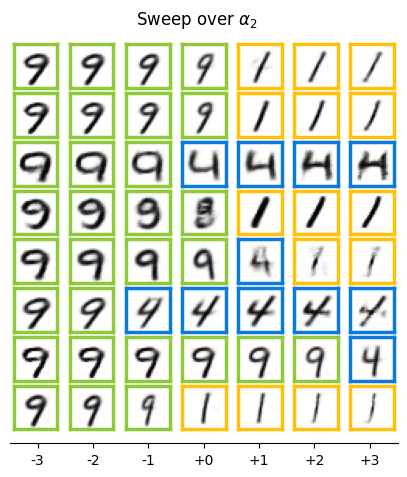
\includegraphics[width=.9\textwidth]{../openreview/pictures/Figure13/alpha_2.png}
		\caption{Sweep $\alpha_2$}
		% \label{fig:beta_1}
	\end{subfigure}
	\begin{subfigure}[t]{.23\linewidth}
		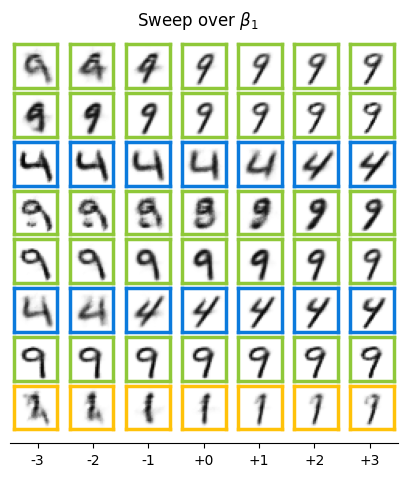
\includegraphics[width=.9\textwidth]{../openreview/pictures/Figure13/beta_1.png}
		\caption{Sweep $\beta_1$}
		% \label{fig:beta_1}
	\end{subfigure}
	\begin{subfigure}[t]{.23\linewidth}
		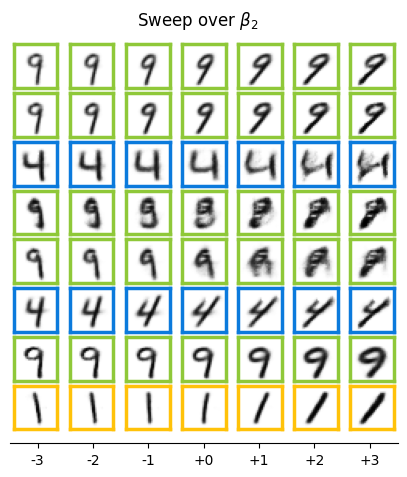
\includegraphics[width=.9\textwidth]{../openreview/pictures/Figure13/beta_2.png}
		\caption{Sweep $\beta_2$}
		% \label{fig:beta_2}
	\end{subfigure}
	
	\caption{Visualizations of learned latent factors for MNIST classifier trained on classes '1' \& '4' \& '9'}
	\label{fig:mnist_results 149 complete}
\end{figure}

\begin{figure}[h]
	\centering
	\begin{subfigure}[t]{.25\linewidth}
		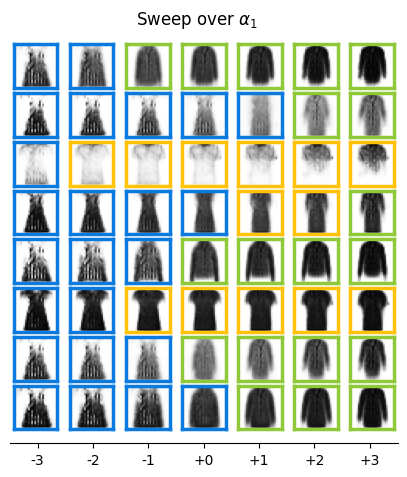
\includegraphics[width=.9\textwidth]{../openreview/pictures/fmnist/alpha_1.png}
		\caption{Sweep $\alpha_1$}
		\label{fig:alpha_1}
	\end{subfigure}
	\begin{subfigure}[t]{.25\linewidth}
		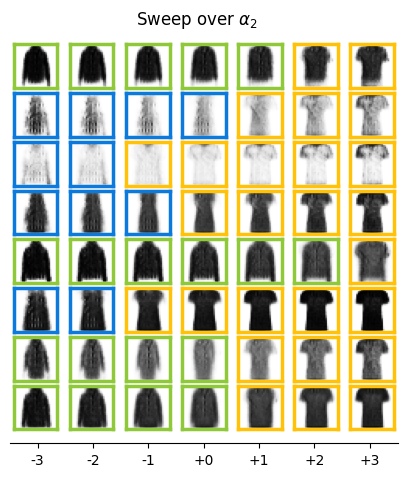
\includegraphics[width=.9\textwidth]{../openreview/pictures/fmnist/alpha_2.png}
		\caption{Sweep $\alpha_2$}
		\label{fig:alpha_2}
	\end{subfigure}
	\begin{subfigure}[t]{.25\linewidth}
		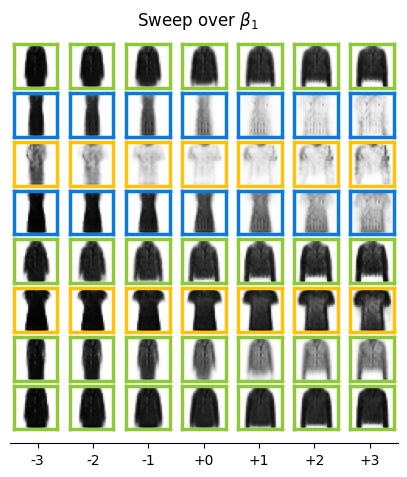
\includegraphics[width=.9\textwidth]{../openreview/pictures/fmnist/beta_1.png}
		\caption{Sweep $\beta_1$}
		\label{fig:beta_1}
	\end{subfigure}
	\begin{subfigure}[t]{.25\linewidth}
		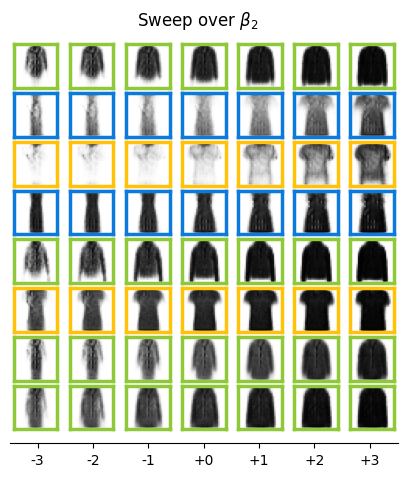
\includegraphics[width=.9\textwidth]{../openreview/pictures/fmnist/beta_2.png}
		\caption{Sweep $\beta_2$}
		\label{fig:beta_2}
	\end{subfigure}
	\begin{subfigure}[t]{.25\linewidth}
		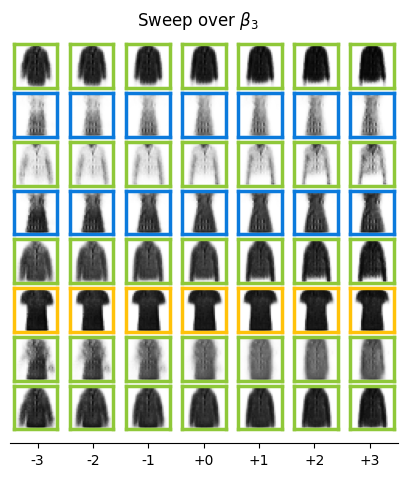
\includegraphics[width=.9\textwidth]{../openreview/pictures/fmnist/beta_3.png}
		\caption{Sweep $\beta_3$}
		\label{fig:beta_3}
	\end{subfigure}
	\begin{subfigure}[t]{.25\linewidth}
		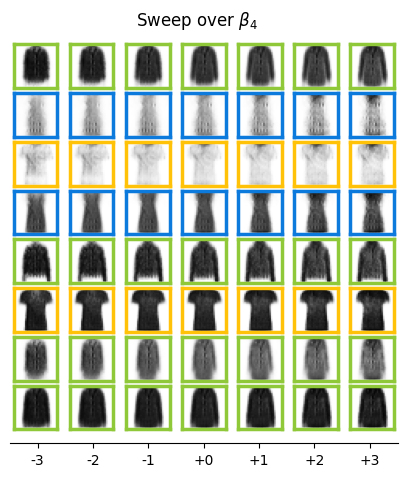
\includegraphics[width=.9\textwidth]{../openreview/pictures/fmnist/beta_4.png}
		\caption{Sweep $\beta_4$}
		\label{fig:beta_4}
	\end{subfigure}
	\caption{Visualizations of learned latent factors for fMNIST classifier trained on classes ‘t-shirt-top,’ ‘dress,’ and ‘coat.’}
	\label{fig:fmnist_results complete}
	
	\begin{subfigure}[t]{.32\linewidth}
		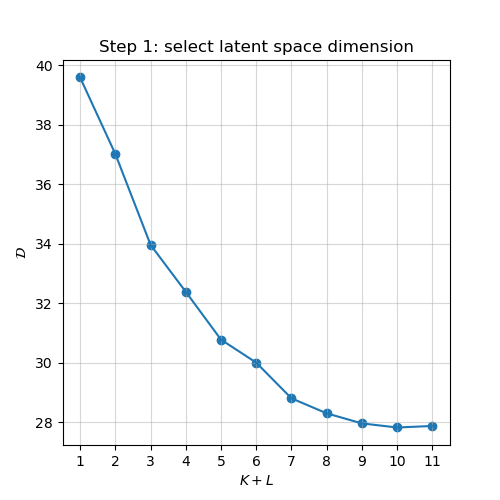
\includegraphics[width=\textwidth]{../openreview/pictures/parameter_search/parameter_search_38_L.png}
	\end{subfigure}
	\begin{subfigure}[t]{.32\linewidth}
		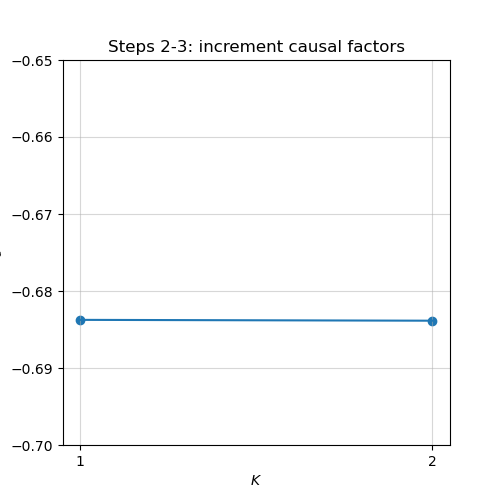
\includegraphics[width=\textwidth]{../openreview/pictures/parameter_search/parameter_search_38_K.png}
	\end{subfigure}
	\begin{subfigure}[t]{.32\linewidth}
		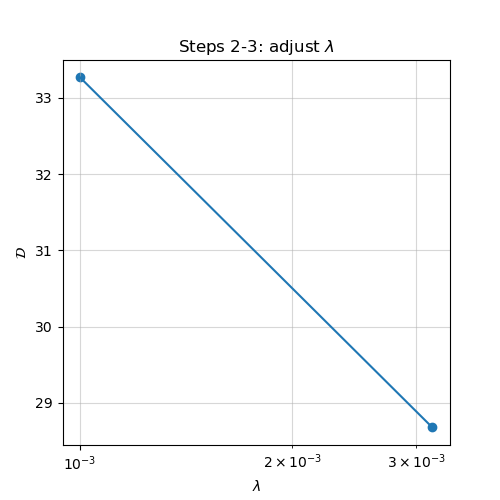
\includegraphics[width=\textwidth]{../openreview/pictures/parameter_search/parameter_search_38_lambda.png}
	\end{subfigure}
	\caption{Results of parameter selection technique for the 3/8 classifier.}
	\label{fig:hparams_38}
	
	\begin{subfigure}[t]{.45\linewidth}
		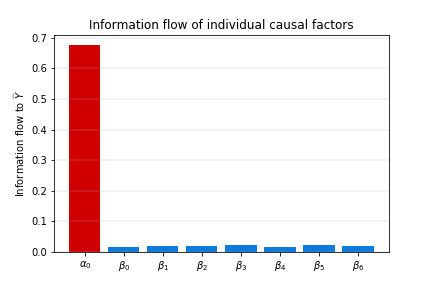
\includegraphics[width=.9\textwidth]{../openreview/ablation_study_38/InformationFlow.png}
		\caption{Information flow 3/8}
		% \label{fig:beta_1}
	\end{subfigure}
	\begin{subfigure}[t]{.45\linewidth}
		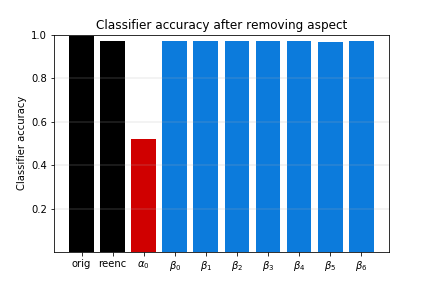
\includegraphics[width=.9\textwidth]{../openreview/ablation_study_38/AblationAccuracy.png}
		\caption{Ablation study 3/8}
		% \label{fig:alpha_1}
	\end{subfigure}
	\begin{subfigure}[t]{.45\linewidth}
		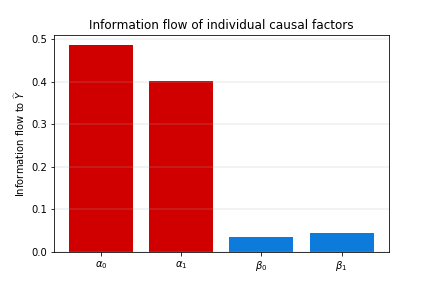
\includegraphics[width=.9\textwidth]{../openreview/ablation_study_149/InformationFlow.png}
		\caption{Information flow 1/4/9}
		% \label{fig:beta_2}
	\end{subfigure}
	\begin{subfigure}[t]{.45\linewidth}
		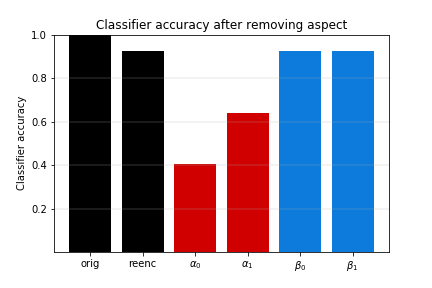
\includegraphics[width=.9\textwidth]{../openreview/ablation_study_149/AblationAccuracy.png}
		\caption{Ablation study 1/4/9}
		% \label{fig:beta_1}
	\end{subfigure}
	\caption{Information flow and ablation study for MNIST dataset.}
	\label{fig:ablation complete}
\end{figure}